\documentclass[chi_draft]{sigchi}

% Use this section to set the ACM copyright statement (e.g. for
% preprints).  Consult the conference website for the camera-ready
% copyright statement.

% Copyright
\CopyrightYear{2017}
%\setcopyright{acmcopyright}
\setcopyright{acmlicensed}
%\setcopyright{rightsretained}
%\setcopyright{usgov}
%\setcopyright{usgovmixed}
%\setcopyright{cagov}
%\setcopyright{cagovmixed}
% DOI
\doi{http://dx.doi.org/10.475/123_4}
% ISBN
\isbn{123-4567-24-567/08/06}
%Conference
\conferenceinfo{IoT}{...}
%Price
\acmPrice{\$15.00}

% Use this command to override the default ACM copyright statement
% (e.g. for preprints).  Consult the conference website for the
% camera-ready copyright statement.

%% HOW TO OVERRIDE THE DEFAULT COPYRIGHT STRIP --
%% Please note you need to make sure the copy for your specific
%% license is used here!
% \toappear{
% Permission to make digital or hard copies of all or part of this work
% for personal or classroom use is granted without fee provided that
% copies are not made or distributed for profit or commercial advantage
% and that copies bear this notice and the full citation on the first
% page. Copyrights for components of this work owned by others than ACM
% must be honored. Abstracting with credit is permitted. To copy
% otherwise, or republish, to post on servers or to redistribute to
% lists, requires prior specific permission and/or a fee. Request
% permissions from \href{mailto:Permissions@acm.org}{Permissions@acm.org}. \\
% \emph{CHI '16},  May 07--12, 2016, San Jose, CA, USA \\
% ACM xxx-x-xxxx-xxxx-x/xx/xx\ldots \$15.00 \\
% DOI: \url{http://dx.doi.org/xx.xxxx/xxxxxxx.xxxxxxx}
% }

% Arabic page numbers for submission.  Remove this line to eliminate
% page numbers for the camera ready copy
% \pagenumbering{arabic}



%% PM Define authornote command for comments
\newcommand{\authornote}[1] {
    \begin{center}
        \framebox{
            {\begin{minipage}[t]{0.9\linewidth}
                \raggedright  \textbf{[PM]}~ \scriptsize #1 \normalsize
            \end{minipage}}
    }
    \end{center}
}

\usepackage{color}
\definecolor{highlight}{rgb}{1,1,0.6}
\definecolor{link}{rgb}{0.5,0.0,0.0}
\definecolor{cite}{rgb}{0.0,0.0,0.6}
\definecolor{url} {rgb}{0.3,0.0,0.3}
\definecolor{grey}{rgb}{0.3,0.3,0.3}


\usepackage[pdftex]{hyperref}
\hypersetup{%
	%pdftitle={\myTitle}, %
	pdfauthor={blind submission}, %
	%pdfkeywords={\programname},%
	bookmarksnumbered, %
	pdfstartview={c}, %
	colorlinks,%
	citecolor=black, %
	filecolor=black, %
	linkcolor=black, %
	urlcolor=black}

\usepackage{soul}
% % annotations environments % % 
\newcommand{\note}[1]{\textit{\textcolor{red}{\{#1\}}}}
\sethlcolor{highlight}

\newcommand{\comment}[2]{\hl{#1} {\color{red}\textit{\{#2\}}}}




\begin{document}
%
% paper title
% Titles are generally capitalized except for words such as a, an, and, as,
% at, but, by, for, in, nor, of, on, or, the, to and up, which are usually
% not capitalized unless they are the first or last word of the title.
% Linebreaks \\ can be used within to get better formatting as desired.
% Do not put math or special symbols in the title.
\title{Mind My Value: a decentralized infrastructure for fair and trusted IoT data pricing}


%\title{\plaintitle}

\numberofauthors{5}
\emptyauthor
%\author{%
%	\alignauthor{Paolo Missier\\
%		\affaddr{Newcastle University}\\
%		\affaddr{Newcastle, UK}\\
%		\email{paolo.missier@newcastle.ac.uk}}\\
%	\alignauthor{Michele Nati\\
%		\affaddr{Digital Catapult}\\
%		\affaddr{London, UK}\\
%		\email{michele.nati@digicatapult.org.uk}}\\
%	\alignauthor{Angelo Capossele\\
%		\affaddr{Digital Catapult}\\
%		\affaddr{London, UK}\\
%		\email{Angelo.Capossele@digicatapult.org.uk}}\\
%	\alignauthor{Andrea Gaglione\\
%	\affaddr{Digital Catapult}\\
%	\affaddr{London, UK}\\
%	\email{Andrea.Gaglione@digicatapult.org.uk}}\\
%	\alignauthor{Shaimaa Bajoudah\\
%	\affaddr{Newcastle University}\\
%	\affaddr{Newcastle, UK}\\
%	\email{S.Bajoudah1@newcastle.ac.uk}}\\
%}


% make the title area
\maketitle

% As a general rule, do not put math, special symbols or citations
% in the abstract
\begin{abstract}
The abstract goes here.
\end{abstract}




\section{Introduction}

Individuals who own and operate IoT edge devices (wearables, smart home etc) should be able to retain some control over the data that is continuously generated by those devices.
Increasingly, such data are considered valuable digital assets that could be traded with third parties:  ``There are third parties that could benefit from using that data, and the challenge is in allowing them to access it under the conditions that data owners find acceptable.'' \note{[Misura, Kresimir, and Mario Zagar. 2016]}

\note{remove this ref from here -- it is now in related work}

Data producers may be, for example, wearables (accelerometers, glucose monitors, heart monitors, smart energy meters in the home), personal, vehicle or home monitoring sensors, etc.
These IoT devices generate various types of data streams, at different rates, which may be of interest to a variety of consumers, typically analytics applications that may operate over data that is aggregated from multiple streams and over time, or on a per-individual basis.
We refer to these consumers generically as Value Added Services (VAS).

In the health sector, for example, individuals' activity levels and fitness data, as recorded by smart phones or dedicated fitness devices, may be of interest to health care providers as well as health insurance companies, even if only in anonymised and aggregate form.
%
In public transport, the density of personal travel card swipes over time at individual metro stations in London will be of interest not only to the transportation authority, but also to taxi companies who need to decide how to position their cars outside metro stations, i.e., in situations where passenger traffic patterns deviate from the predictable norm.
%
 Similarly, aggregate smart metering is shown to enable providers to optimise the delivery of commodity services, eg water, energy.  \note{CITE}.
%
As a final sports example, today it is possible to quantify an athlete's effort during a competition using a number of wearable devices, from bio-harness to accelerometers, to video feeds. 
It is easy to imagine that, in the near future, athletes may be able to license these feeds to followers who are interested in tracking their competition online.

Underlying all these examples is the emergent idea that data streams produced by IoT devices that belong to individuals or organisations are increasingly viewed as \textit{tradeable assets} with a potential market value.
%
Indeed,  a number of models are emerging on how to price online data, and data marketplaces already exist in a number of scenarios \note{CITE}.
%
In this paper we explore the idea of a marketplace specifically for IoT data, which enables device owners not only to control the distribution of the data produced by their devices, but also to trade them with third parties.
%
Specifically, we focus on a ``IoT Big Data trading'' scenario where high Velocity, high Volume and potentially high Variety data streams flow from IoT edge devices, the producers, to VAS, typically embodied as cloud services located in the core network.

As in any marketplace, IoT data trading should be governed by an agreed-upon set of rules, set in advance, which determine what kinds of contract and transactions are acceptable, and stipulate sanctions when the rules are violated.
%
While we acknowledge that contractual agreements must be stipulated between the individuals or organisations that own or control the devices and the VASs, in this work we are only concerned with the study of the underpinning technology that makes it possible to realise IoT data trading, by enhancing the current IoT infrastructure and regardless of specific pricing and contract models.

The main novel element of our work is that we challenge the common assumption that a marketplace must be controlled by a trusted authority, in charge of certifying the identity of the participants, and ensuring fairness. 
In particular, data brokers typically play the role of trusted network components that are controlled by a marketplace authority.
%
In contrast, we envision a decentralized and self-regulating marketplace where rules are automatically enforced,  fairness of the transactions guaranteed, and sanctions imposed in response to violations.
%

\note{use this to refer to emerging business models for data marketplaces -- \cite{Stahl2016} Stahl, F., Schomm, F., Vossen, G., \& Vomfell, L. (2016). A classification framework for data marketplaces. Vietnam Journal of Computer Science, 3(3), 137–143. https://doi.org/10.1007/s40595-016-0064-2}

\note{\cite{7004800} Perera, C., Liu, C. H.,\& Jayawardena, S. (2015). The Emerging Internet of Things Marketplace From an Industrial Perspective: A Survey. IEEE Transactions on Emerging Topics in Computing, 3(4), 585–598. https://doi.org/10.1109/TETC.2015.2390034\\
	A comprehensive survey of industry-ready IoT technology -- good to support the claim that there are a lot of sensor types out there, but ``marketplace''  here just means, HW that is on the market...}

%
An 2012 survey of data vendors \cite{Schomm2013} includes 46 data suppliers. While the definition of data marketplace used in the paper is generic (``a platform on which anybody can upload and maintain data sets, with license-regulated access to and use of the data'') and geared towards static data, like Microsoft’s Azure Data Market, it should be possible to extend the classification of marketplace types to \textit{data in movement}, and IoT data streams in particular, which is our focus.

\note{general background -- can't find a place for this, it's one of many possible examples. \cite{7113786} Islam, S. M. R., Kwak, D., Kabir, M. H., Hossain, M., \& Kwak, K. S. (2015). The Internet of Things for Health Care: A Comprehensive Survey. IEEE Access, 3, 678–708. https://doi.org/10.1109/ACCESS.2015.2437951}




\subsection{Contributions}

In the rest of the paper we present our approach to addressing some of the challenges that emerge when trying to realise such a trust-less IoT data marketplace.

Our first contribution is a data architecture for tracking data flows through brokers, using a publish-subscribe pattern, or through network servers, to achieve granular metering of IoT data exchanges.

Secondly, we explore the use of blockchain technology and \textit{Smart Contracts} \cite{SMART-CONTRACTS} to remove the need for centralised trust. We discuss the challenges and limitations of using Smart Contracts for automatic dispute resolution.

Finally, we present a prototype realisation of the marketplace, using MQTT brokers for granular data exchange with added traffic metering capabilities, and the Ethereum Smart Contracts technology for enforcing the contracts definition and providing dispute resolution capabilities.

In our initial evaluation we show that smart contracts are indeed a viable option for validation of contract compliance, and assess its capability to handle a stream of blockchain transactions at varying arrival rate.

\subsection{Background and Related work}

%%%%
% sensors as service
%%%%
%\note{   \cite{Perera2014}  Perera, C., Zaslavsky, A., Christen, P., \& Georgakopoulos, D. (2014). Sensing as a service model for smart cities supported by Internet of Things. Transactions on Emerging Telecommunications Technologies, 25(1), 81–93. https://doi.org/10.1002/ett.2704}

%\note{ \cite{distefano2012sensing}  Distefano, S., Merlino, G., \& Puliafito, A. (2012). Sensing and actuation as a service: A new development for clouds. In Network Computing and Applications (NCA), 2012 11th IEEE International Symposium on (pp. 272–275). }

%\note{Banerjee, P., Friedrich, R., Bash, C., Goldsack, P., Huberman, B., Manley, J., … Veitch, A. (2011). Everything as a Service: Powering the New Information Economy. Computer, 44(3), 36–43. https://doi.org/10.1109/MC.2011.67}

The idea of considering data from IoT sensors as tradeable assets is closely related to that of \textit{Sensing as a Service} (SaaS) models, or even \textit{Sensing and Actuation as a service} (SAaaS) \cite{distefano2012sensing}, themselves derivatives of the more general ``Everything as a Service'' (XAAS) cloud-based model for data exchange \cite{5719575}. Perera et al. \cite{Perera2014}, for instance, outline a vision of a near future for Smart Cities, where data streams emanating from pervasive Internet of Things sensors are accessible through services. The SaaS model consists of four conceptual layers: sensors and their owners, sensor publishers, service providers, and sensor data consumers. In this classification, our work is relevant to all of these agents, as it enables fair and metered data exchanges amongst sensors owners and publishers on one side, and sensor data consumers, on the other.


%%%%
%\note{related: data pricing}
%%%%
%\note{\cite{Li:2014:TPP:2691190.2691191} Li, C., Li, D. Y., Miklau, G., \& Suciu, D. (2014). A Theory of Pricing Private Data. ACM Trans. Database Syst., 39(4), 34:1--34:28. https://doi.org/10.1145/2691190.2691191}

%\note{\cite{7437020} Niyato, D., Hoang, D. T., Luong, N. C., Wang, P., Kim, D. I., \& Han, Z. (2016). Smart data pricing models for the internet of things: a bundling strategy approach. IEEE Network, 30(2), 18–25. https://doi.org/10.1109/MNET.2016.7437020}

%\note{related: trust management}
%\note{ \cite{Bao:2012:DTM:2378023.2378025} Bao, F., \& Chen, I.-R. (2012). Dynamic Trust Management for Internet of Things Applications. In Proceedings of the 2012 International Workshop on Self-aware Internet of Things (pp. 1–6). New York, NY, USA: ACM. https://doi.org/10.1145/2378023.2378025}

%\note{\cite{Yan2014a} Yan, Z., Zhang, P., \& Vasilakos, A. V. (2014). A survey on trust management for Internet of Things. Journal of Network and Computer Applications, 42, 120–134. https://doi.org/10.1016/j.jnca.2014.01.014}
%

Our traffic monitoring infrastructure assumes that suitable pricing models that associate values to messages are in place.
However, it is agnostic and ``orthogonal'' to the specific pricing model, as long as the price of a complex bundle of data offering can be expressed in terms of unit cost associated to individual messages. 
Thus, in principle, any of the existing models for data pricing may be used in combination with traffic metering. Such models, recently proposed, range from theoretical frameworks for assigning prices to query answers as a function of their accuracy \cite{Li:2014:TPP:2691190.2691191}, to adaptations of \textit{Smart Data Pricing} \cite{Sen:2015:SDP:2847579.2756543} to the dynamic pricing of IoT data, such as personal data from wearable sensors \cite{7437020}.

A trust management model should also be established, i.e., to enable self-regulation of marketplace rules as we briefly discuss at the end of the paper.
Again, while this is out of our scope, existing frameworks can be used on top of out infrastructure.
Yan et al \cite{Yan2014a} provide a starting point, by exploring the notion of trust across the IoT platform layers (physical sensing, network, and application layer), with focus on  a wide range of properties from security to goodness, strength, reliability, availability, ability of data. Interestingly, however, their survey largely overlooks issues of trust amongst participants in a data marketplace, i.e., in the context of data exchange transactions.

%\note{ Roman, D., \& Stefano, G. (2016). Towards a Reference Architecture for Trusted Data Marketplaces: The Credit Scoring Perspective. In 2016 2nd International Conference on Open and Big Data (OBD) (pp. 95–101). IEEE. https://doi.org/10.1109/OBD.2016.21}
More directly useful in our setting, as we progress in our work, is Roman and Gatti's study of trust in data marketplaces \cite{7573695}, based on \textit{credit scoring}, where a direct connection is made to the use of blockchain technology in connection with data trading.

%%%%
%\note{related: marketplace for data}
%%%%

Two technical architectures for data marketplaces are directly relevant to our work.
%\note{ Schomm, F., Stahl, F., \& Vossen, G. (2013). Marketplaces for Data: An Initial Survey. SIGMOD Rec., 42(1), 15–26. https://doi.org/10.1145/2481528.2481532}
%\note{\cite{Cao:2016:MMR:2926746.2883611}  Cao, T.-D., Pham, T.-V., Vu, Q.-H., Truong, H.-L., Le, D.-H., \& Dustdar, S. (2016). MARSA: A Marketplace for Realtime Human Sensing Data. ACM Trans. Internet Technol., 16(3), 16:1--16:21. https://doi.org/10.1145/2883611}
Firstly the MARSA platform \cite{Cao:2016:MMR:2926746.2883611}, designed specifically to deal with real-time data streams by interacting with existing IoT platforms.
The motivation for this work is very similar to ours, namely to provide a marketplace where owners have an incentive to trade their data, for either personal or community benefit.
The many technical requirements that emerge from analysis of data marketplace potential translate into a complex architecture, which includes data flow orchestration, participants registration, data contract management, and payment.  
While these components do address complex marketplace requirements, our main challenge, namely to remove the need for a central trusted authority to manage the marketplace and ensure its fairness, remains unique to our work.

Secondly, Misura, K., \& Zagar \cite{7765669} focus on a query-based mechanism, whereby devices register their data supply capabilities to a broker along with a number of properties, and consumers express interest in data streams by querying those properties. The broker then connects the supplier stream to the consumer, and monitors usage. 
This is relevant work, as this type of matching of consumer data requirements to suppliers capabilities is more sophisticated than simple topic subscription.
In our future work we plan to move away from fine-grained data subscription and towards complex data contracts (bundles), as discussed briefly at the end of the paper.

%\note{ Misura, K., \& Zagar, M. (2016). Data marketplace for Internet of Things. In 2016 International Conference on Smart Systems and Technologies (SST) (pp. 255–260). IEEE. https://doi.org/10.1109/SST.2016.7765669}


%\note{\cite{7146004} Blazquez, A., Tsiatsis, V., \& Vandikas, K. (2015). Performance Evaluation of OpenID Connect for an IoT Information Marketplace. In 2015 IEEE 81st Vehicular Technology Conference (VTC Spring) (pp. 1–6). IEEE. https://doi.org/10.1109/VTCSpring.2015.7146004}

	
\section{Brokered IoT data as tradeable assets}

We denote the set of producers (IoT devices) and consumers (VAS) that participate in the marketplace as $P = \{p_1 \dots p_n \}$ and $C = \{ c_1 \dots c_m \}$, respectively.
	In line with common IoT platforms practices, we are going to assume that data exchanges between any $p_i$ and any $c_j$ are mediated by one ore more brokers. 
This follows a commonly used publish/subscribe model for data streams, whereby the $p_i$ act as publishers and the $c_j$ are subscribers.
A set $T = \{ t_1 \dots t_r \}$ of topics is agreed upon by all participants (i.e., publishers and subscribers), 
%
We also assume, in line with common practice, that topics are organised into a hierarchy, with '/\#' used to mean ''all topics``. 
For example, leaf-level topics may be ''heart rate``,''GPS track``, ''glucose reading``, ''energy reading`` and so forth. Note that topics are the only type of descriptive metadata associated with the messages. 
%
Each data stream generated by each $p_i$ can be segmented into discrete messages, and each message has an associated topic $t_k$.

In our marketplace model, a contractual agreement between $p_i$ and $c_j$ is defined by a set $T_{ij} \subset T$ of topics and a time window $ W = [w_s, w_e] $, with the interpretation that $p_i$ agrees to let all its messages tagged with any $t \in T_{ij}$ reach $c_j$ for the duration of $W$, and $c_j$ agrees to pay a corresponding data licensing fee. 

While a variety of pricing models have recently been proposed for digital assets in emerging data marketplace scenarios \note{CITE}, discussing how the marketplace sets the data prices is beyond the scope of this work. 
Instead, we are simply going to assume that each individual message is a digital asset with a constant unit value $\mathit{val}(t_k)$, which is determined solely by the message's topic $t_k$.

This setting is represented in \note{some part of...} Fig. \ref{fig:reference-architecture}, where for simplicity we show one single broker that manages all $c_j$ subscriptions and thus is responsible for routing message from each $p_i$.
%
Gateways are responsible for mapping raw device data streams to a publisheable message stream, including generating appropriate topics.
In our testbed deployment we use MQTT brokers, and the gateways generate messages by encapsulating either a batch of the raw data stream or an aggregation of it, depending on the type of stream, into the MQTT payload.


\begin{figure}
	\centering
	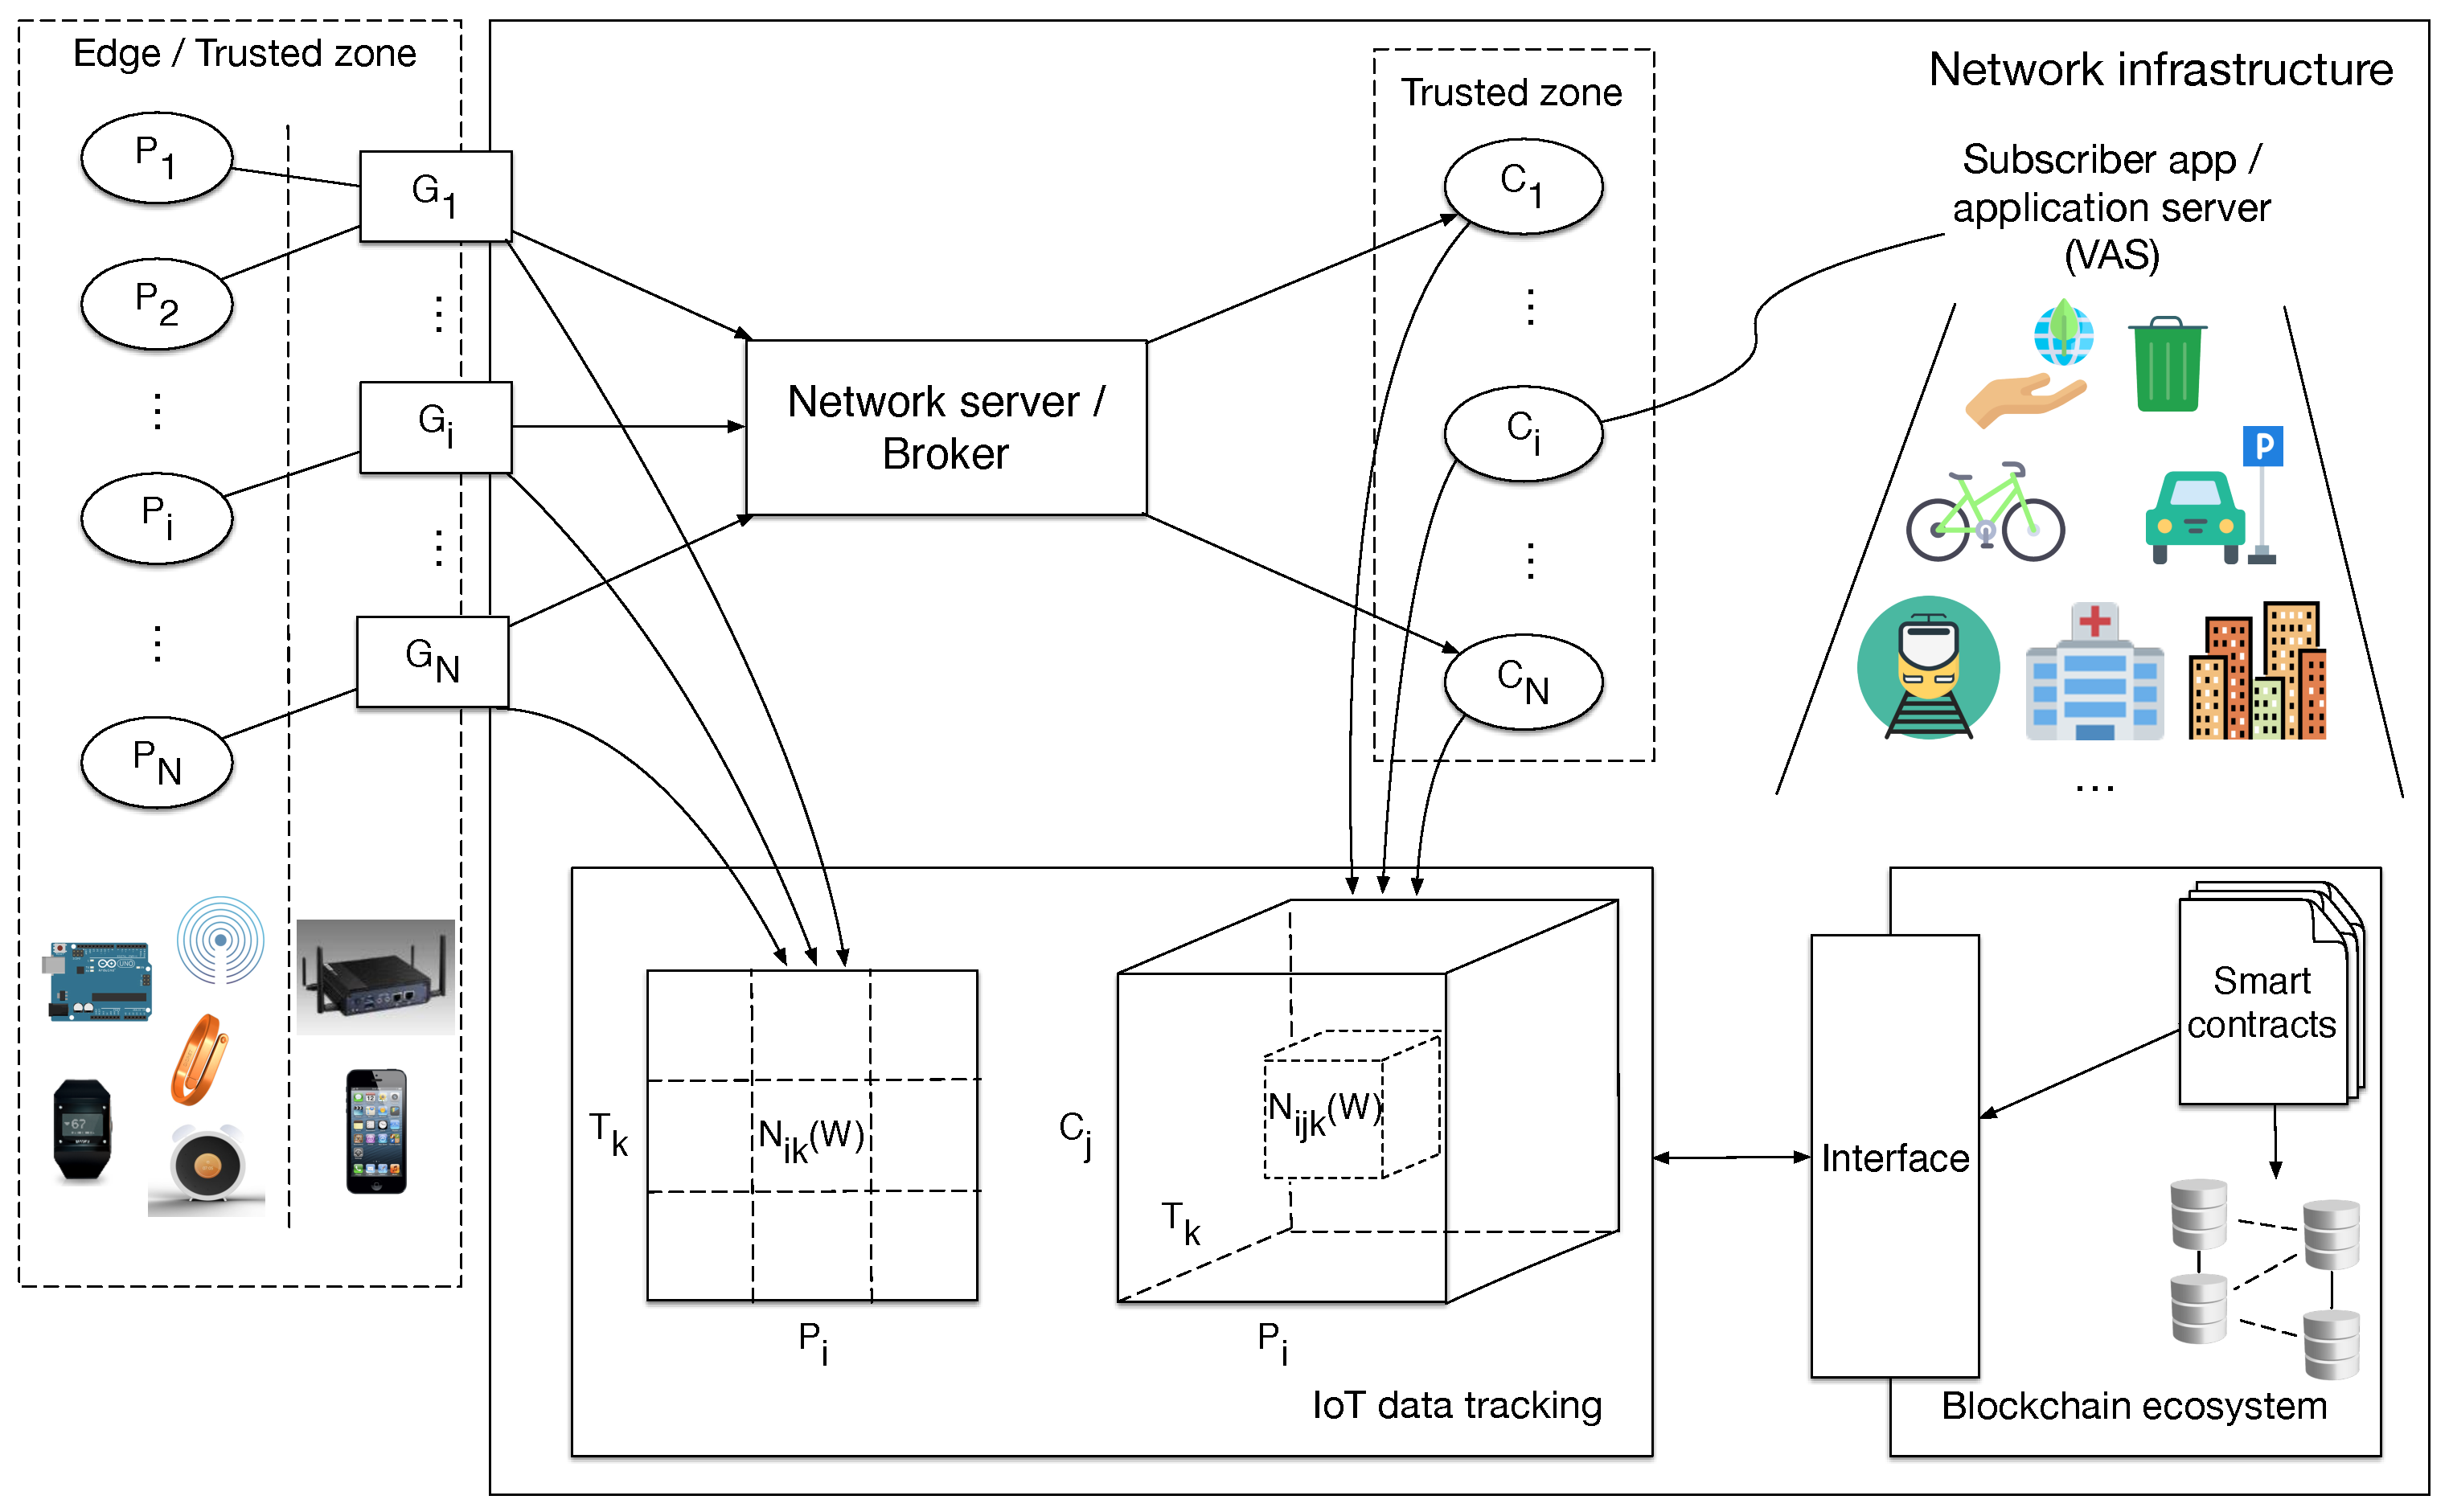
\includegraphics[width=\columnwidth]{figures/IoT-tracking-arch-2}
	\caption{Reference architecture for decentralised IoT data traffic metering based on blockchain and Smart Contracts}
	\label{fig:iot-tracking-arch-2}
\end{figure}

In the standard pub/sub model, publishers and subscribers are unaware of one another, and their interaction is entirely mediated by the broker. 
To enable explicit marketplace interactions, we implement a variation of the model whereby every message topic embeds the publisher's ID, which in combinatio with MQTT's topic regular expressions capability enables a subscriber to selectively choose the stream they intend to license.
For example, device ``1234'' may publish messages about a specific room's temperature using topic  \#/temperature/1234/living\_room\_temperature. 
A publisher may choose to subscribe to this specific topic, or to any  living\_room\_temperature message using expression \#/temperature/*/living\_room\_temperature, or to any generic temperature message from ``1234'' or from any subscriber.

Note incidentally that the model includes the case, not shown in the figure, where a VAS may aggregate data from multiple $ p_i $s and then publish this value-added data, enabling other VAS to license it. 
In this case, a VAS is both a consumer and a producer.

\subsection{Centralised Traffic metering}

This model enables many-many agreements between any subsets of $P$ and $C$, with pricing that is determined by $T$.
Suppose the broker is trusted with \textit{metering} all traffic, that is, monitoring and logging all message flows for a time interval $W$, and suppose that a number of agreements are active between pairs of $p_i$ and $c_j$ during $W$.
Let 
\[N_{ijk}(W) = \mathit{count}(p_i, c_j, t_k)\]
denote the number of messages about topic $t_k$ that originated from $p_i$ and reached $c_j$ during $W$.
Ideally, at the end of $W$ the broker will be able to determine the reward that $p_i$ is due by each $c_j$, as a simple function of $N_{ijk}(W)$ and unit costs $\mathit{val}(t_k)$:
\begin{equation}
\mathit{reward}(p_i, W) = \sum_{\substack{t_k \in T \\ c_j \in C}} N_{ijk}(W) \cdot \mathit{val}(t_k)
\label{eq:reward}
\end{equation}
(note that $N_{ijk}(W = 0$ if $c_j$ does not subscribe to $t_k$).

\subsection{Traffic cubes and settlement}

Thus, in this ideal scenario data flows easily translate into a set of payment settlement transactions involving pairs $(p_i, c_j)$.
In our testbed we realise this capability by extending a Mosquitto MQTT broker so it logs each message routing event as a tuple into a \textit{TrackerDB} database:
$ \langle p_i, c_j, t_k \rangle $

At the end of each $W$, the log is aggregated over each $p_i \in P, c_j \in C, t_k \in T$, resulting in a set of tuples that we call a \textit{traffic cube}:
\begin{equation}\label{eq:cube}
\mathit{cube}(W) = \{ \langle p_i, c_j, t_k, N_{ijk}(W) \rangle \}_{p_i \in P, c_j \in C, t_k \in T}
\end{equation}
Here we borrow our terminology from OLAP database practice where a  ``cube'' is a table with $ N $ attributes, in which the first $ N-1 $ attributes are  dimensions in a database schema (in our case, these are the Producers, Consumers, and Topics) and the last is an aggregation over values in the database for each combination of the dimensions -- in our case, a count().
We use a matrix indexing notation to refer to specific cells in the cube, i.e.:
%where some of the $i,j,k$ are fixed, to denote specific slices of the cube, for example:
\[ \mathit{cube}(W)[p_i, c_j, t_k] = N_{ijk}(W) \] 
%denotes the set $  \{ \langle p_i, c_j, t_k, N_{ijk}(W) \rangle \}_{c_j \in C, t_k \in T} $ of all tuples for a set $p_i$.
%Similarly, \[ \mathit{cube}(W)[p_i, -, t_k]\] 
%is the set 
%$  \{ \langle p_i, c_j, t_k, N_{ijk}(W) \rangle \}_{c_j \in C} $, and so forth.

A traffic cube contains a summary  of all data flows observed by a broker. Notice that these cubes only contain \textit{metadata}, i.e., the counts, but they disregard the content of the messages.
%
Cubes are used for settlement either by the broker itself, or by a trusted third party service. Fig. \note{xx} summarises this basic architecture, as it is realised in our testbed. 
We use a Cassandra NoSQL database for the \textit{TrackerDB}, to ensure scalability. 
A traffic reporting service generates traffic cubes on demand by querying the \textit{TrackerDB}, in response to requests issued by client applications (including possibly independent third party clients). The service is accessible through a REST interface.

\begin{figure}
	\fbox{Basic cubes figure}
	\caption{Broker-generated traffic cubes}
	\label{fig:cubes}
\end{figure}

\textit{Settlement} is the process of calculating a set of balances $ \mathit{bal}(c_j, p_i, W) $, that is, the fractions of total reward owed by each $c_j$ to each $p_i$ at the end of each $W$:
\begin{equation}
\mathit{bal}(c_j, p_i, W) = \sum_{t_k \in T} N_{ijk}(W) \cdot \mathit{val}(t_k)
\label{eq:balance}
\end{equation}

In the centralised scenario we have considered so far, settlement is straightforward, as we have assumed that we have complete visibility of the entire traffic over time, and that the cubes are complete and correct.
Note that, under the same trust assumptions, settlement extends easily to a more realistic scenario where multiple brokers are deployed, each enhanced with the same logging capabilities and local traffic reporting service.

This centralised scenario becomes challenging, however, if we remove the assumption that the broker is the only central element that is responsible for settling payments.
We now present an extended model where individual participants may be metering the portions of data flows that are visible to them, and settlement occurs by collecting and analysing the reports from each participant, at the end of each time period $W$.

\section{Removing the need  for trust in the data flow network}  \label{sec:no-trust}

Any marketplace where the reward model is based on message counts is vulnerable to malicious behaviour by any of the participants. Specifically, the suppliers (the publishers) have an incentive to claim to have produced more messages than they have in reality, while conversely, subscribers have an incentive to under-report the number of messages they receive.
%
If we remove the assumption that the broker(s) are trusted, we must also accept that they may be prepared to collude with any of the participants, and thus deliver traffic cubes that may not be correct or complete.
Discovering such collusions may not be possible when the broker is the only source of traffic counts available to the settlement service.  At the same time, resolving any disputes amongst pairs of participants requires a public and irrefutable record of the reported traffic.

To address these problems we rely on two over-arching principles: (1) personal responsibility of each participant in the marketplace, which shall report their own counts of messages sent (publishers) or received (subscribers), and (2) transparency, whereby these reports are posted as part of immutable and verifiable blockchain transactions.
In practice, we propose a two-steps approach.
%

Firstly, we remove the assumption that traffic cubes are generated by the broker alone, and instead enable networks elements close to the publishers and to the subscribers, i.e., gateways and VAS respectively, to generate the cubes.
%
Secondly, we adopt emerging consensus-based distributed transaction ledgers, specifically blockchain and Smart Contract technology, to realise the settlement service.
As we explain in more detail later (Sec. \ref{sec:blockchain}), Smart Contracts extend the standard blockchain transaction model by adding the capability to execute arbitrary code, which operates on data structures contained in the transaction itself. 
In this case, a transaction that is initiated at the end of each window $W$ may operate on the traffic cubes that participants make available at the end of $W$.
This  approach provides at the same time transparency and accountability, because the content of the blockchain is public and can be inspected, and a way to address disputes, because for each window W, multiple (partial) views of each cube are made available to the settlement service.

\subsection{Unilateral traffic cubes} \label{sec:u-cubes}

Traffic cubes that are generated by the broker summarise the entire traffic during $W$.
In contrast, traffic summaries generated by marketplace participants reflect the \textit{local} views of each participant in the data exchanges.
These are therefore necessarily partial and incomplete, as each participant, unlike the broker, has no visibility of the end-to-end data flows. 
We denote these as \textit{unilateral} traffic cubes, defined as follows.

We assume that a producer does not know which VAS subscribe to its stream, while subscribers, in contrast, know the source of the messages they receive. 
Let $\mathit{sub}(t_k) \subseteq C $ denote the set of subscribers to $t_k$.

A \textit{publisher's cube} $\mathit{cube^p}$ is a slice of a complete traffic cube, for a specific producer $p_i$ and without the consumer dimension:
\[
\mathit{cube}^p(W, p_i)  =  \{ \langle t_k,  N^s_{ik}(W) \rangle \}_{t_k \in T}
\]
where $N^s_{ik}(W)$ is the count of messages with topic $t_k$ sent by $p_i$ during $W$.

As subscribers know the source of the messages they receive, we may assume that a subscriber will produce summary reports that include the publisher dimension, but which only contain the tuples that pertain to a single $c_j$. We refer to this as a \textit{subscriber's cube}, $ \mathit{cube^s} $, defined as follows:
\[
\mathit{cube^s}(W, c_j)  =  \{ \langle p_i, t_k, N_{ijk}(W) \rangle | c_j \in \mathit{sub}(t_k)\}_{p_i \in P, t_k \in T}
\]

\subsection{Consistency and settlement with unilateral cubes}

Suppose that, at the end of $W$, every $p_i$ and $c_j$ produce  unilateral cubes relative to $W$. 
These form the set
\begin{equation}\label{eq:all-cubes}
\{ \mathit{cube}^p(W, p_i) \}_{p_i \in P}\cup \{\mathit{cube^s}(W, c_j) \}_{c_j \in C} 
\end{equation}
As each of these cubes provides a partial view of the same complete cube that would have been generated centrally by a broker, we expect that the values found in these cubes must somehow be consistent with such global cube.

The pub/sub model implies that the number of messages sent by $p_i$ with topic $t_k$ during $W$ must be equal (assuming no messages are lost and ignoring duplicate transmissions) to the number of messages each $c_i$ that subscribes to $t_k$ receives from $p_i$. 
We can capture this constraint formally using our cubes notation, as follows.
%
For each $ p_i \in P, t_k \in T, c_j \in \mathit{sub}(t_k)$:
\begin{equation}\label{eq:cubes-consistency}
\begin{split}
& \mathit{cube}^p(W, p_i)[t_k] = N^s_{ik}(W) = \\
& \mathit{cube}(W)[p_i, t_k, c_j]  = N_{ijk}(W) = \\
& \mathit{cube^s}(W, c_j)[p_i, t_k]
\end{split}
\end{equation}

%\begin{definition}
We say that the set (\ref{eq:all-cubes}) of all unilateral cubes is \textit{consistent} at $W$, if and only their contents satisfy constraint (\ref{eq:cubes-consistency}).
%\begin{end}
We use this definition as a basis for settlement of message exchanges within each $W$, in the general case that the broker cannot be trusted to provide a single global cube that is complete and correct.
%
Specifically, in our architecture we  now assume that a new, independent component receives all cubes in (\ref{eq:all-cubes}) at the end of each $W$, and checks their consistency using (\ref{eq:cubes-consistency}). 
In the next section we discuss a practical implementation of this idea, where this new component is realised as a Ethereum Smart Contract and unilateral cubes are posted publicly as part of blockchain transactions. As explained in more detail later, a Smart Contract is a script that operates on the blockchain. It can be viewed as a third party trusted service, because its implementation is transparent and agreed upon by all marketplace participants. 

In this decentralised scenario, such a settlement service must be able to deal with two inter-dependent issues, namely (1) \textit{completeness} and (2) \textit{consistency} of the set (\ref{eq:all-cubes}) of all cubes.

The case when set (\ref{eq:all-cubes}) is both complete and consistent is straightforward and results in successful settlement, as all information for settlement is available, and there are no disagreements.

When the set of cubes is incomplete, we may try to use (\ref{eq:cubes-consistency}) to propagate missing values from the more complete to the less complete cubes. 
More precisely, suppose $ \mathit{cube}^p(W, p_i) $ is missing for a $p_i$.
If $ N_{ijk}(W) = \mathit{cube^s}(W, c_j)[p_i, t_k] $ is available for some $t_k$ and some $ c_j \in \mathit{sub}(t_k) $, then we set $  \mathit{cube}^p(W, p_i)[t_k]=  N_{ijk}(W) $.
In practice, this can be viewed as ``taking $ c_j $s word for $p_i$s missing report''.

Symmetrically, the settlement service may use the available $ \mathit{cube}^p(W, p_i)$, in combination with subscription information $ \{\mathit{sub}(t_k) | t_k \in T \}$, to fill in missing values in 
$  \mathit{cube^s}(W, c_j)  $, i.e., by setting 
$ \mathit{cube^s}(W, c_j)[p_i, t_k]  =  \mathit{cube}^p(W, p_i)[t_k]$ for each $t_k$ and each $c_j \in \mathit{sub}(t_k)$.

Of course, there is no guarantee that all missing values can be propagated. 
In this case, settlement for the $\langle p_i, c_j \rangle$ pairs corresponding to the missing cube entries is simply not possible.

The final, and perhaps more important case occurs when constraint (\ref{eq:cubes-consistency}) is violated for some combination of $\langle p_i, c_j, t_k \rangle$.
This may occur because producers have an incentive to over-report the number of messages they sent, while symmetrically, subscribers have an incentive to under-report the number of messages they received.

Either of these malicious scenarios manifests itself as inequalities in (\ref{eq:cubes-consistency}), of the form:
\begin{equation}\label{eq:inconsistencies}
\mathit{cube}^p(W, p_i)[t_k] > \mathit{cube^s}(W, c_j)[p_i, t_k]
\end{equation}
In this situation, we are able to detect the inconsistency, but we may not have enough information to determine whether $p_i$, $c_j$, or both are guilty of malicious behaviour.
Such determination is beyond the scope of this paper, but in the final discussion section we present initial ideas on promoting a self-regulating marketplace in the presence of malicious behaviour.

In our initial implementation, described in the next section, the settlement service simply reports the detected inequalities.

\section{Initial proof-of-concept realisation}  \label{eq:realisation}


\subsection{Blockchain and Smart Contracts}  \label{sec:blockchain}

\note{cite in blockchain section}

\note{	\cite{Swan}  Swan, M. (n.d.). Blockchain : blueprint for a new economy.}

\note{\cite{Buterin2014} Buterin, V. (2014). A next-generation smart contract and decentralized application platform. Retrieved from http://buyxpr.com/build/pdfs/EthereumWhitePaper.pdf}


The second element of our approach is based on the use of emergin Blockchain and Smart Contracts tecnhology.

\note{FIXME -- still a dump of Michele's text . background}

Blockchain is essentially a distributed ledger of information (e.g., a transaction from A to B in the bitcoin world), a copy of which cannot be arbitrarily altered without being spotted and for which consistency of each information can be achieved in a decentralized and distributed way, without requiring trust in any third party. These properties, that in the bitcoin world provides a very strong business case (e.g., removing transaction costs associated to clearinghouse functionalities when transferring money), can also provide a trust case for exchanging access to different assets, without requiring trust among parties.

Decentralized Applications (DApps) use assets and services from different sources, not controlled by only one entity (in contrast to the traditional centralized client/server web). Using smart contracts and off-chain information makes more practical to develop new DApps. s-Health apps can be seen as a particular type of DApps. Bitcoin is the first DApp built on top of the blockchain: it is a digital and interoperable currency (i.e., it does not require conversion across the world), using the blockchain infrastructure and some complex cryptographic algorithms, to achieve (nearly) zero transaction fees while avoiding the double-spending problem (e.g., possibility to spend a given amount twice) and without requiring to trust in any third party to police this risk. Thinking about the value of different assets, bitcoin and alt-coin (i.e., bitcoin plus metadata) can provide an interoperable and open cross-domain incentives platform for redistributing the value created from assets sharing, transparently covering the interests of all the involved assets providers.

Blockchain has been later leveraged to manage Smart Contracts, small pieces of software that encode a set of conditions and actions that a machine can interpret and that can be executed as expected using the blockchain infrastructure without third party involvement or supervision \cite{Buterin2014}. These functionalities can be interesting when it comes to give permission to access different assets (datasets and devices) only for specific purposes.

Blockchain is usually adopted by Decentralized Autonomous Organizations (DAOs), which require neither written statements nor physical governance bodies, to run on code expressed by a set of Smart Contracts. This concept is interesting for organizations where different stakeholders can vote and agree on the rules for sharing their assets, e.g., for particular social benefits or research purpose, thus deciding how their rewards should be distributed while influencing and supporting the creation of specific s-Health services. Through DAOs, the principles, rules and benefits deriving from data sharing can be distributedly enforced without requiring any trusted third party. While this is a powerful concept to achieve autonomy and avoid misuse, particular attention is required in order to properly encode the right human assisted governance structure in the DAOs. This might require a governance body that supervises the rules implemented as DAO by an open developers community, following a rigorous, open, transparent and accounted review process.


\note{ANDREA}


\authornote{We need reference to ETH architecture, with APIs call and a snippet of the code. We can add some numbers on how much this will cost to run and consequently set up a minimum cost for each data in order to keep infrastructure sustainable.
Logic: “data” is a “count cube”. The platform generates a stream of these cubes at a certain rate, which is tunable using the window size on the TrackerDB. The arrival rate of the cubes determines the frequency at which contracts are executed, and therefore the cost over time.
}

\section{Evaluation and Lessons learnt}

\authornote{
\note{new from Michele}

	\begin{itemize}
\item test assuming no need of settlement, value are the same
\item Test different time periods for cube generation, fine grained vs to larger interval, up to daily
\item Invariance wrt to period for cube computation 
\item Dependency wrt to number of sources and VAS (not addressed here)
	\end{itemize}
}


\authornote{
\note{old list}
	\begin{itemize}
		\item Are smart contracts an adequate implementation model to realise a fair marketplace?
\item Are there limitations in the reconciliation phase?
\item Cost of operating and marketplace: executing transactions and how to control them -- contract activated in an adaptive mode.  Who owns the contracts?  (ideal answer: nobody. Participants share the cost of transactions)
\item Scalability: how the cubes decouple the data flow rates from the transaction frequency
\item Data marketplace model is preliminary and not validated on real world use cases. It is based on minimal data semantics (ie the topic) and has no notion of more sophisticated contract models.
	\end{itemize}
}


\authornote{
\note{lessons learnt}

	\begin{itemize}
\item event vs time series, costs and requirements
\item Liability of oracolize model for trust; requirements of new interfaces
\item Volatility of market and price
	\end{itemize}
}


\section{Conclusion and future work}




% conference papers do not normally have an appendix


% use section* for acknowledgment
\section*{Acknowledgment}


The authors would like to thank...

\bibliographystyle{IEEEtran}
\bibliography{IEEEabrv,iot-conf}



% trigger a \newpage just before the given reference
% number - used to balance the columns on the last page
% adjust value as needed - may need to be readjusted if
% the document is modified later
%\IEEEtriggeratref{8}
% The "triggered" command can be changed if desired:
%\IEEEtriggercmd{\enlargethispage{-5in}}

% references section

% can use a bibliography generated by BibTeX as a .bbl file
% BibTeX documentation can be easily obtained at:
% http://mirror.ctan.org/biblio/bibtex/contrib/doc/
% The IEEEtran BibTeX style support page is at:
% http://www.michaelshell.org/tex/ieeetran/bibtex/
%\bibliographystyle{IEEEtran}
% argument is your BibTeX string definitions and bibliography database(s)
%\bibliography{IEEEabrv,../bib/paper}
%
% <OR> manually copy in the resultant .bbl file
% set second argument of \begin to the number of references
% (used to reserve space for the reference number labels box)




% that's all folks
\end{document}


